\begin{equation}
	\rho\left(E\right) = \frac{1}{\pi}\lim_{\epsilon \to 0^+} \mathrm{Im}\mathrm{Tr}\op{G}\left(E + i\epsilon\right)
	\label{green:densityeq}
\end{equation}
\begin{figure}[H]
	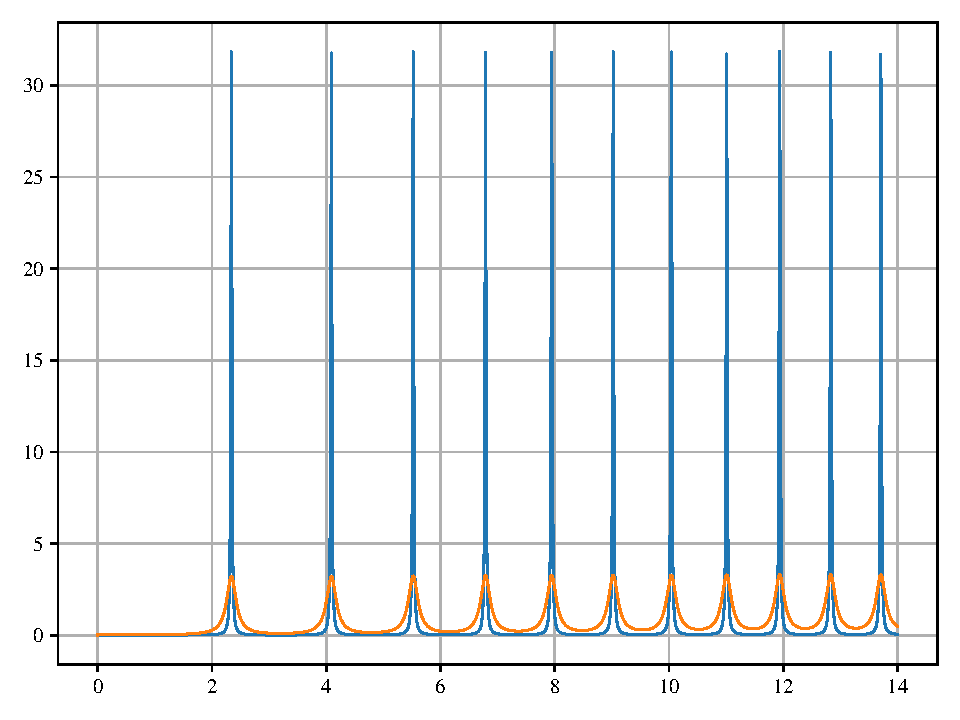
\includegraphics[scale=1]{./figs/dosfromgreen.pdf}
	\caption[Állapotsűrűség]{\Aref{green:densityeq}. képlet alapján számolt állapotsűrűség. A kék függvényt $\epsilon = 10^{-3}/b$, a narancssárga görbét pedig $\epsilon = 10^{-2}/b$ helyettesítéssel kaptuk. Látható, hogy $\epsilon$ csökkentésével a tüskék egyre keskenyebbek, és egyre magasabbak lesznek.}
	\label{green:állapotsűrség}
\end{figure}
\begin{figure}[H]
	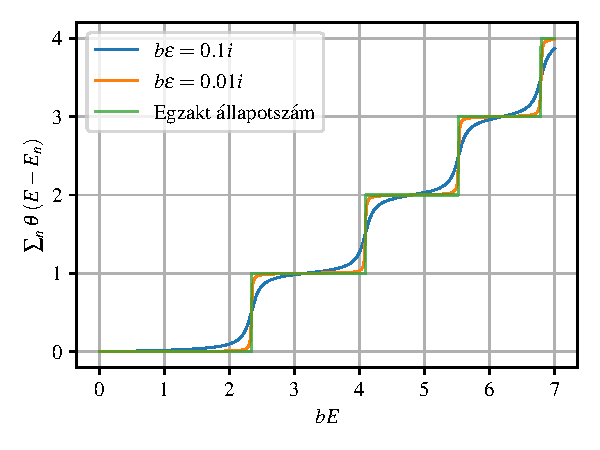
\includegraphics[scale=1]{./figs/numberofstatesfromgreen.pdf}
	\caption[Állapotok száma]{\Aref{green:állapotsűrség}. ábrán bemutatott függvények integrálja látható ezen az ábrán. Mind a két függvény ugrása közelítőleg $1$, ami at jelenti, hogy \aref{green:állapotsűrség}. ábrán látható tüskék alatti terület jó közelítéssel $1$. Az $\epsilon$ csökkentése a lépcsőfüggvényhez közelíti az integrált függvényt, ami egyezik az elvárásokkal.}
\end{figure}